Demonstration of Selenium using php-webdriver by Facebook on top of PHPUnit.
\subsection{Prerequisites}
\label{prerequisites}

Make sure your server (computer) meets the following requirements:

\begin{itemize}
\item PHP $>$= 5.6.4 (server (\texttt{apache2} or \texttt{nginx}) is \textbf{not required})

\item composer (how to install \href{https://getcomposer.org/doc/00-intro.md#installation-linux-unix-osx}{guide}\footnote{\href{https://getcomposer.org/doc/00-intro.md\#installation-linux-unix-osx}{https:/\slash getcomposer.org\slash doc\slash 00-intro.md\#installation-linux-unix-osx}})

\item npm (how to install \href{https://docs.npmjs.com/getting-started/installing-node}{guide}\footnote{\href{https://docs.npmjs.com/getting-started/installing-node}{https:/\slash docs.npmjs.com\slash getting-started\slash installing-node}})

\item \href{http://selenium-release.storage.googleapis.com/index.html?path=3.0/}{selenium-standalone-server 3.0.1 [\ensuremath{\sim}20MB]}\footnote{\href{http://selenium-release.storage.googleapis.com/index.html?path=3.0/}{http:/\slash selenium-release.storage.googleapis.com\slash index.html?path=3.0\slash }}

\item browser specific drivers (whole list can be found \href{http://www.seleniumhq.org/download/}{here}\footnote{\href{http://www.seleniumhq.org/download/}{http:/\slash www.seleniumhq.org\slash download\slash }} in section \emph{Third Party Browser Drivers})

\begin{itemize}
\item \href{https://sites.google.com/a/chromium.org/chromedriver/}{chromedriver}\footnote{\href{https://sites.google.com/a/chromium.org/chromedriver/}{https:/\slash sites.google.com\slash a\slash chromium.org\slash chromedriver\slash }} - Google Chrome

\item \href{https://github.com/mozilla/geckodriver/releases}{geckodriver}\footnote{\href{https://github.com/mozilla/geckodriver/releases}{https:/\slash github.com\slash mozilla\slash geckodriver\slash releases}} - Mozilla Firefox

\item \href{https://github.com/SeleniumHQ/selenium/wiki/SafariDriver}{safaridriver}\footnote{\href{https://github.com/SeleniumHQ/selenium/wiki/SafariDriver}{https:/\slash github.com\slash SeleniumHQ\slash selenium\slash wiki\slash SafariDriver}} - Safari

\item \href{https://developer.microsoft.com/en-us/microsoft-edge/tools/webdriver/}{edgedriver}\footnote{\href{https://developer.microsoft.com/en-us/microsoft-edge/tools/webdriver/}{https:/\slash developer.microsoft.com\slash en-us\slash microsoft-edge\slash tools\slash webdriver\slash }} - Microsoft Edge

\item \href{https://github.com/operasoftware/operachromiumdriver}{operadriver}\footnote{\href{https://github.com/operasoftware/operachromiumdriver}{https:/\slash github.com\slash operasoftware\slash operachromiumdriver}} - Opera

\end{itemize}

\end{itemize}

\begin{quote}
\textbf{Note}: I tested this working example only with \textbf{chromedriver}\\
\textbf{Note}: on Mac OS you can install \textbf{selenium-standalone-server} (and some drivers) using \href{http://brew.sh/index.html}{homebrew}\footnote{\href{http://brew.sh/index.html}{http:/\slash brew.sh\slash index.html}}
\texttt{
brew install selenium-server-standalone
brew install chromedriver
}
\end{quote}

\subsection{Installation \&\& setup}
\label{installationsetup}

\begin{itemize}
\item install php dependencies using composer

\item install Todo application using npm

In terminal change working directory to \texttt{.\slash application} and run following:

\begin{verbatim}
composer install
composer dump-autoload -o
npm install
\end{verbatim}
\item serve \texttt{.\slash application\slash index.html}; two options are available (remember which one you used)

\begin{itemize}
\item set up server and serve using virtual-host
\item use \texttt{file://\slash $<$path to application folder$>$\slash index.html}
\end{itemize}
\item manually test working Todo application you should see following:
\end{itemize}

\begin{figure}[htbp]
\centering
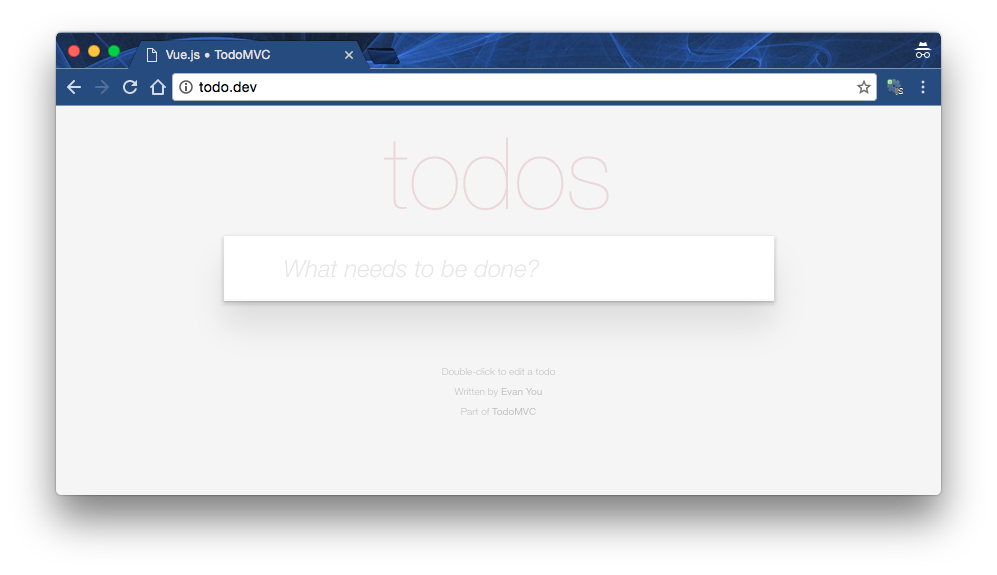
\includegraphics[keepaspectratio,width=\textwidth,height=0.75\textheight]{img/vue-js-todo.png}
\end{figure}

\begin{quote}
\textbf{Note}: I am using apache2 and vhost to serve static page on local domain \emph{todo.dev}
\end{quote}

After package managers install all required software you are ready to use example code.

\subsection{Usage \slash  running tests}
\label{usagerunningtests}

Change \texttt{\$url} variable on \href{https://github.com/Kyslik/asos-selenium/blob/master/application/tests/TodoApp/TodoAppTest.php#L11}{TodoAppTest.php on line 11}\footnote{\href{https://github.com/Kyslik/asos-selenium/blob/master/application/tests/TodoApp/TodoAppTest.php\#L11}{https:/\slash github.com\slash Kyslik\slash asos-selenium\slash blob\slash master\slash application\slash tests\slash TodoApp\slash TodoAppTest.php\#L11}} to reflect path to Todo application.

Open up two terminal windows (or tabs), one is going to be used for \textbf{selenium-standalone-server} (tab A) and second one is going to be used for \textbf{PHPUnit} (tab B). 

\begin{itemize}
\item in tab A start \textbf{selenium-standalone-server} on port 4444 (default), to do so run following:
 \texttt{
 java -jar $<$path\_to$>$\slash selenium-server-standalone-$<$version$>$.jar
}
 $>$\textbf{Note}: on Mac OS if you used homebrew to install selenium-standalone-server you can run following:
 \texttt{
 selenium-server -port 4444
}
\item in tab B change working directory to \texttt{.\slash application} and simply run \texttt{vendor\slash bin\slash phpunit}
\end{itemize}

\subsection{Brief explanation}
\label{briefexplanation}

In tab A you can monitor what exactly is PHPUnit invoking while test is beeing run (kind of selenium log).
In tab B you may observe execution of PHPUnit test suite located in \texttt{.\slash application\slash tests\slash TodoApp}. 

On the background PHPUnit invokes selenium-standalone-server with some rules\slash patterns and selenium-standalone-server translates it to (in this case) chromedriver API.